Particle accelerators were first developed in the early 20th century as a tool for high-energy physics research. By increasing particles' energy they allow us to investigate the subatomic structure of the world and to study the properties of the elementary particles and the fundamental forces. On a basic level, accelerators increase the energy of charged particles using electric fields. Through the years significant technological progress has been achieved resulting in higher energies and greatly enhanced performance of the machines. Additionally, various types of accelerators have been developed (cyclotrons, linacs, synchrotrons etc) using different types of particles (hadrons or leptons) and their use was also expanded in other fields such as medicine and industrial research. 
% Brief history of particle accelerators: https://cds.cern.ch/record/261062/files/p1_2.pdf
% Summary for accelerators: https://www.energy.gov/articles/how-particle-accelerators-work#:~:text=There%20are%20two%20primary%20roles,charged%20particles%20for%20medical%20treatment.



\section{The CERN accelerator complex}

CERN (European Organisation of Nuclear Research), located on the Franco-Swiss border near Geneva, is at the forefront of the accelerator physics research as it operates an extensive network of accelerators, illustrated in Fig.~\ref{fig:cern_accelerator_complex}, including the well-known Large Hadron Collider (LHC)~\cite{Brüning:782076}.

LHC is a circular machine, 27\, km long, built about 100\,m underground and is currently the largest and most powerful accelerator. It accelerates and collides two counter-rotating beams of protons or ions (circulating in two different rings) at the four main experiments which are located around the LHC ring, namely ATLAS, CMS, ALICE and LHCb. The highlight of CERN and of the LHC operation up to now was the discovery of the Higgs boson in 2012 from ATLAS~\cite{ATLAS_Higgs} and CMS~\cite{CMS_Higgs}, from proton collisions at 3.5\,TeV (center-of-mass energy of 7\,TeV), which was a milestone for the standard model. % Importance of higgs discovery: https://home.cern/resources/faqs/cern-and-higgs-boson

The beams used by the LHC are produced and gradually accelerated by the injector chain which is a sequence of smaller machines boosting the energy of the beam. In particular, Linac4 (which replaced Linac2 in 2020) accelerates the protons up to 160\,MeV, the Proton Synchrotron Booster (PSB) up to 2\,GeV, the Proton Synchrotron (PS) up to 26\,GeV and the the Super Proton Synchrotron (SPS) up to 450\,GeV. Finally, the protons are injected in the LHC where they are accelerated up to the collision energy of 6.5\,TeV (center-of-mass energy of 13\,TeV). It should be noted, that LHC delivered collisions with center-of-mass energy of 7\,TeV during Run 1 (2010-2013) which was increased to 13\,TeV for the Run 2 (2015-2018) and for Run 3 (2020-present). 
% actually from april 2012 till the end of run 1 it deleveled 8 TeV. 

\begin{figure}[!h] %https://cds.cern.ch/images/CERN-GRAPHICS-2022-001-1
    \centering         
    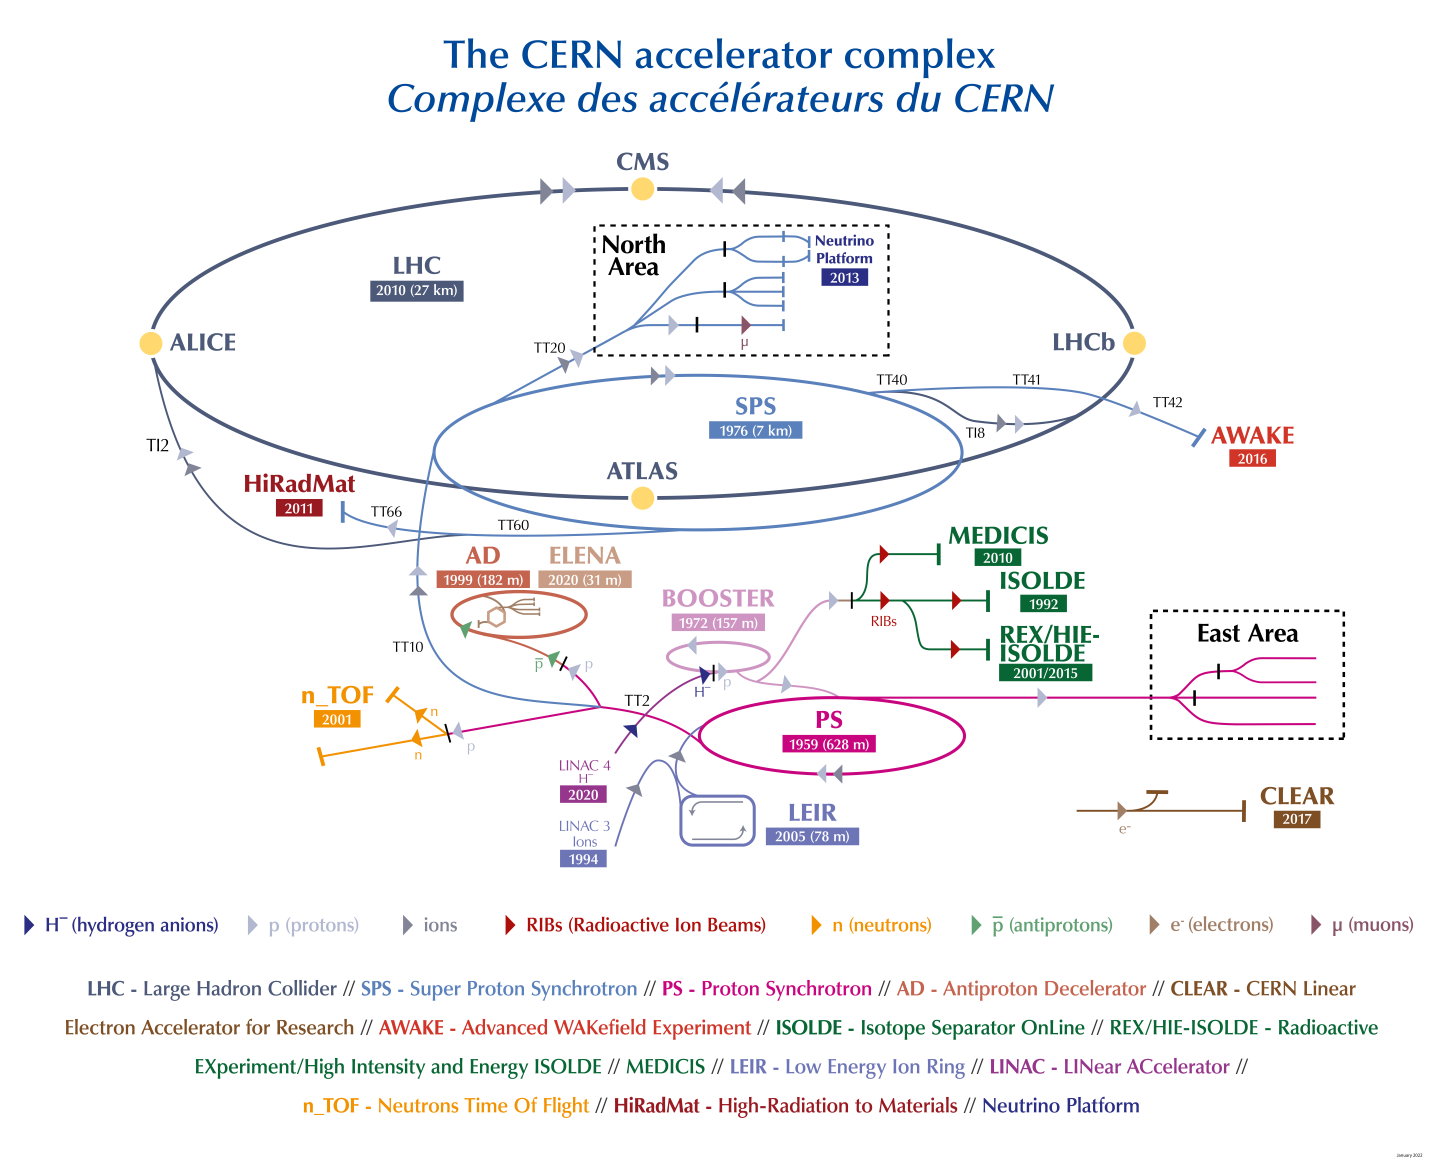
\includegraphics[width=1\textwidth]{images/introduction/cern_accelerator_complex.png}
        \caption{Schematic view of the CERN accelerator complex. The different colors correspond to the different machines. The year of commissioning and the type of particles used in each one of them are also indicated along with the circumference for the circular machines. The image is courtesy of CERN.}
        \label{fig:cern_accelerator_complex}
 \end{figure}

 It is worth mentioning that not only protons but also lead ions are accelerated in the LHC, starting their journey from Linac3 and LEIR and then following the same route as proton beams.


 Finally, the accelerators in the injector chain not only prepare the beam for the LHC but also provide beams to various other facilities and experiments at lower energies. Examples are the Anti-proton Decelerator (AD) which studies antimatter, the Online Isotope Mass Separator (ISOLDE) which studies the properties of the atomic nuclei using radioactive beams, and the Advanced Proton Driven Plasma Wakefield Acceleration Experiment (AWAKE) which investigates particle acceleration by proton-driven plasma wakefields.

 \subsection{The CERN Super Proton Synchrotron}
 % sps history: https://be-dep-op-sps.web.cern.ch/history
 The majority of the research described in this thesis was conducted for the Super Proton Synchrotron (SPS). Thus, some additional information about this machine is provided here. The SPS (shown with light blue color in Fig.~\ref{fig:cern_accelerator_complex}) was first commissioned in 1967 and has a circumference of 6.9\,km. It used to operate as a proton-antiproton collider ($\mathrm{Sp\bar{p}S}$) and later on as an injector for the Large Electron Positron collider (LEP) while it also provided beams for fixed-target experiments (e.g. in the North Area). Even though the SPS can accelerate various particle types (protons, antiprotons, electrons, and heavy ions) the following information will concern its operation with proton beams which is the topic of the research presented in this thesis.

 Currently, the SPS is the second biggest accelerator at CERN and it can accelerate protons from 26\,GeV up to 450\,GeV. Due to its past use as a collider, it can also operate as a storage ring. This operational mode is called "coast" and was used for the majority of the experimental studies presented in this thesis. During coast, the bunches circulate in the machine for long periods at constant energy. The highest energy at which SPS can operate in coast is 270\,GeV. 

 %After that they are injected in the LHC. Hoewever, as it used to be a collider it can operate as a storage ring, it is called coast (des ti exeis grapsei.) and will be used for the studies in this thesis.
 



\section{High-Luminosity LHC project and Crab Cavities}
%LHC is the flagship of the CERN accelerator complex and is the at the cutting edge of the accelerator and high energy physics research with almost ten thousand scientists working for and with it. In order to extend its discovery potential LHC will undergo a major upgrade in the coming years. 
% Hl-lhc book: p.2 hl-lhc is the top priority of the european strategy of particle physics. 
High-Luminosity LHC (HL-LHC)~\cite{HL_LHC_yellow_report, Brning2015} is the upgrade of the LHC machine which will extend its potential for discoveries. In particular, it aims to increase the instantaneous luminosity by a factor of 5 beyond the current operational values and the integrated luminosity by a factor of 10. 

The luminosity, along with the energy, is a key parameter defining the performance of a collider as is a measure of the collision rate. The instantaneous luminosity is expressed as~\cite{luminosity}:

\begin{equation}\label{eq:luminosity_inst}
    \mathcal{L} = \frac{n_b f_\mathrm{rev}N_1 N_2}{4 \pi \sigma_x \sigma_y} \frac{1}{\sqrt{1+(\frac{\sigma_z}{\sigma_\mathrm{xing}} \frac{\theta_c}{2})^2}},
\end{equation}

where $\frev$ is the revolution freuency of the machine, $n_b$ is the number of colliding bunch pairs, $N_{1,2}$ is the number of particles per bunch, $\sigma_{x,y}$ is the transverse beam size at the interaction point, $\sigma_z$ the rms bunch length, $\sigma_{\mathrm{xing}}$ the transverse beam size in the crossing plane and $\theta_c$ is the full crossing angle between the colliding beams. % Andy's comment: use "number of particles per bunch" instead of "bunch intensity" which is slightly ambiguous.
 The crossing angle, is often introduced between the bunches in a collider to reduce parasitic collisions and get rid of the remnants after the collision. For reference, in the LHC, the crossing angle has order of magnitude $10^{-4}$ radians. % hundreds of micro radians, see sofia's thesis Table 4.4 for example. https://cds.cern.ch/record/2743602/files/CERN-THESIS-2020-169.pdf

The integrated luminosity is the one that ultimately defines the performance of the machine as it provides the total number of recorderd events. It depends both on the instantaneous luminosity and on the machine availability. The integrated luminosity, is expressed as~\cite{HL_LHC_yellow_report}:
\begin{equation}\label{eq:integrated_luminosity}
    \mathcal{L}_I \equiv \int_{\Delta t} \mathcal{L} dt,
\end{equation}

where $\mathcal{L}$ is the instantaneous luminosity as defined in Eq.~\eqref{eq:luminosity_inst}.
% for more details and specific values check sofias thesis.
% and: https://accelconf.web.cern.ch/ipac2015/papers/thxb2.pdf

HL-LHC aims to achive instantaneous luminosity of $\mathcal{L} \sim 5 \cdot 10^{34} \ \mathrm{cm^{-2} s^{-1}}$ and an increase on the integrated luminosity from 300 $\mathrm{fb^{-1}}$ to 3000 $\mathrm{fb^{-1}}$ over its lifetime of 10-12 years~\cite{Brunning_Rossi}. 
% The integrated luminosity for both lhc and hl-lhc is over 10-12 years.

% Source v2: https://accelconf.web.cern.ch/ipac2019/papers/mopgw095.pdf

%\normalsize{\textbf{Crab Cavities}}\\
\subsection{Crab cavities}\label{subsec:CC_intro}
To achieve its luminosity goals, HL-LHC will employ numerous innovative technologies. Crab cavity technology (will be denoted as $\CC$ in this thesis)~\cite{Calaga:2673544} is one of the key componenets of the project as it will be employed to restore the luminosity reduction caused by the crossing angle, $\theta_c$ (see Eq.~\eqref{eq:luminosity_inst}).

A crab cavity is an RF cavity which provides a transverse, sinusoidal like, kick to the particles depending on their longitudinal position within the bunch. A graphical visualisation of the kick is shown in Fig.~\ref{fig:cc_simple_kick}. It can be seen that the head (leading part) and the tail (trailing part) of the bunch receive opposite deflection while the particles at the center remain unaffected.

\begin{figure}[!h] % at the directory of ipac22
    \centering         
    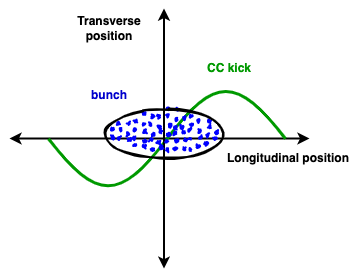
\includegraphics[width=0.5\textwidth]{images/introduction/sin_CC_kick_LHC_beams.drawio.png}
        \caption{Visualisation of the CC kick (green line) on the bunch particles (blue dots). The bunch here appears much smaller than the CC wavelength which means that only the linear part of the kick affects the bunch. This will be the case for the HL-LHC scenario.}
        \label{fig:cc_simple_kick}
 \end{figure}

The $\CC$s will be installed in the two main interaction points of LHC, ATLAS and CMS. According to the plan, four $\CC$s will be installed on each side of the interaction points (two for each ring). This is displayed in Fig.~\ref{fig:LHC_layout_CCs} with the red (ATLAS) and orange (CMS) markers. The reason why two $\CC$s are needed in each ring on each side of the IP is discussed in the following paragraphs (local vs global scheme).

\begin{figure}[!h] % made at diagrams.net saved at google docs
    \centering         
    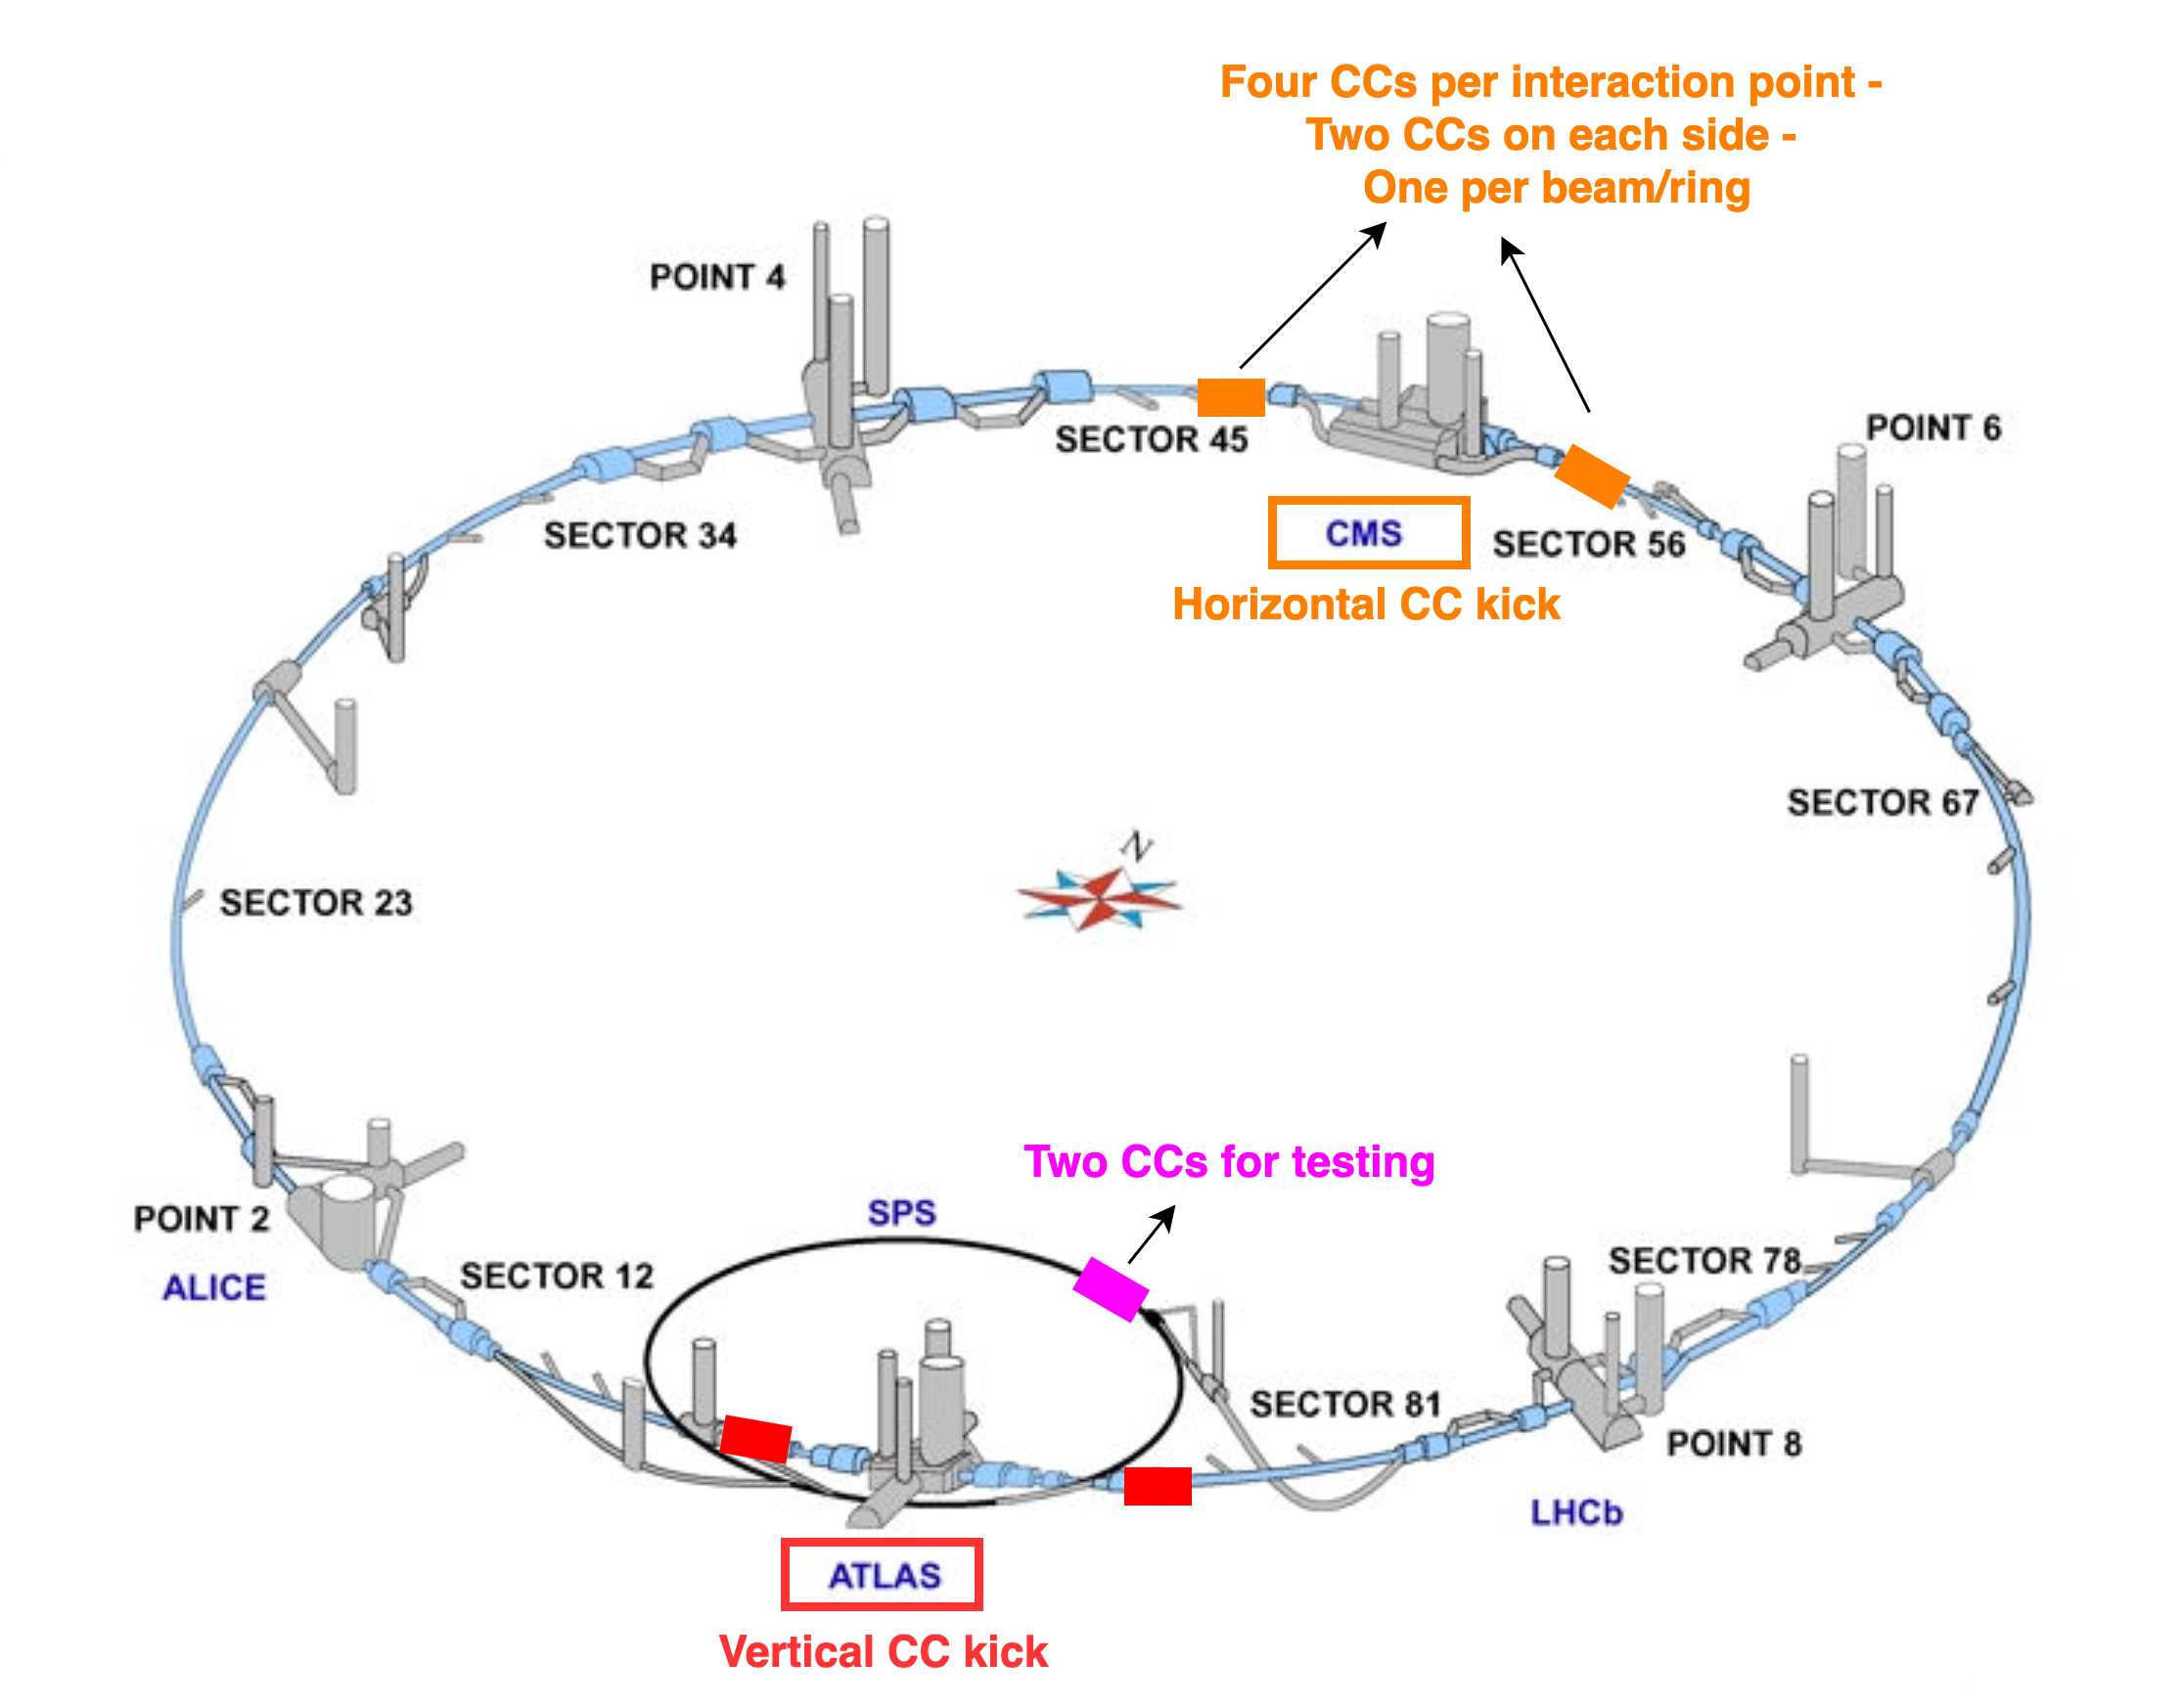
\includegraphics[width=0.8\textwidth]{images/introduction/LHC_layout_CCs.png}
        \caption{Layout of the LHC and the SPS. The CC location for the HL-LHC configuration is marked. Two CCs (one per ring) will be installed on each side of ATLAS (red) and CMS (orange). Two protoype CCs were also installed in the SPS (magenta) in 2018, to be tested before their installation in LHC. The layout can be found in Ref.~\cite{LHC_SPS_layout} and was modified inspired by Ref.~\cite{LHC_SPS_layout_v2}.}
        \label{fig:LHC_layout_CCs}
 \end{figure}

In this configuration, the bunches receive the transverse deflection from the first pair of $\CC$s just before reaching the interaction point. This results in a rotation of the bunch, which mitigates the crossing angle and restores the head-on collisions. The deflection is cancelled once the bunches reach the second pair of $\CC$s which are symmetrically placed at the opposite side of the interaction point. The collision of the bunches in the presence of the $\CC$s is illustrated in Fig.~\ref{fig:crossing_with_and_without_CCs}~\cite{Verdú-Andrés:2263119}.
% 90 deg between CCs and IP. https://cds.cern.ch/record/2263119/files/10.1016_j.nuclphysbps.2015.09.025.pdf

\begin{figure}[!ht]
    \centering
    \begin{subfigure}[t]{0.45\textwidth}
        \centering
        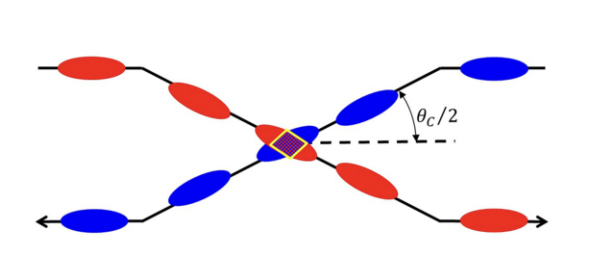
\includegraphics[width=1\textwidth]{images/introduction/no_crab_crossing.png}
        \caption{Crossing without CCs}
        %\label{fig:add_label_here}
    \end{subfigure}
    \hfill
    \begin{subfigure}[t]{0.45\textwidth}
        \centering
        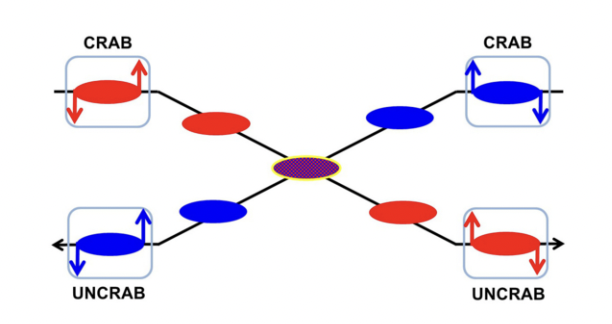
\includegraphics[width=1\textwidth]{images/introduction/crab_crossing.png}
        \caption{Crossing with CCs}
        %\label{fig:add_label_here}
    \end{subfigure}
    \hfill
     \caption{Collision with and without the use of CCs~\cite{Verdú-Andrés:2263119}. CCs restore the overlap between the bunches recovering the luminosity reduction caused by the crossing angle, $\theta_c$. The blue and red colors indicate indicate two bunches in the different rings.} 
     \label{fig:crossing_with_and_without_CCs}
 \end{figure}


% Local vs global CC scheme: https://slideplayer.com/slide/10896302/ 
The above scheme, with $\CC$s before and after the interaction point, is called the local crabbing scheme. An alternative scheme, named the global crabbing scheme, was also under discussion in the first stages of the project. In such as scheme, the closed orbit distortion that is caused by the fact that the head and the tail of the bunch are kicked in opposite directions propagates in the ring, resulting in transverse bunch oscillations~\cite{Brning2015}. This scheme is cost-efficient compared to the local scheme as it only requires two CCs. However, it introduces significant constraints on the betatron phase advance between the interaction points and the CCs. The constraints are enhanced by the fact that the bunch crossing in ATLAS takes place in the vertical plane while in CMS in the horizontal. To this end, the local CC scheme was chosen for the HL-LHC configuration. % uncrabbing.
%HL-LHC book p.138: The transverse kick introduced by this cavity, different  for  the  head  and  the  tail  of  each  bunch,  is  equivalent  to  a  closed  orbit  distortion, i.e. head and tail would follow their individual closed orbit around the ring, their tilt wobbling around the unperturbed closed orbit of the bunch center.

In order to accommodate the crossing in both transverse planes two $\CC$ designs have been developed: the Double-Quarter Wave (DQW) and the RF dipole (RFD), which provide vertical and horizontal deflection respectively. Information on their design can be found in Refs.~\cite{Zanoni:2288282, DeSilva:2288607, Xiao:1992565, Verdú-Andrés:2113440}

% short summary about KEKB in sylivias paper: https://cds.cern.ch/record/2263119/files/10.1016_j.nuclphysbps.2015.09.025.pdf
The $\CC$s have already been successfully used in the KEKB collider in Japan, during 2007-2010, with lepton beams ($e^{+} - e^{-}$)~\cite{CC_KEKB_4440798, Funakoshi:1955812, oide:pac07-mozaki01}. However, there are significant differences in the beam dynamics in the presence of $\CC$s in leptons and hadrons (HL-LHC case). One of the most crucial points is the impact of errors (e.g. RF noise) which leads to beam degradation~\cite{Calaga:2773279, Alekou:2696109}. This is not an issue of concern for lepton beams as they nevertheless experience emittance damping due to synchrotron radiation. For proton beams, the synchrotron radiation damping is much weaker meaning that the beam degradation can lead to emittance growth which eventually can result in loss of luminosity. % Andy's comment: "emittance damping" would be better than "beam-size damping". 

% other crabbing errors: phase and amplitude rf noise, wakefields (Calaga)
% other difference between letptons and protons (protons: much longer bunches)

% Potential questions to answer for the CC test.
%https://indico.cern.ch/event/800428/attachments/1804664/2945632/CrabCavity_BE_Seminar.pdf
As the $\CC$s have never been used with protons before, two prototype superconducting $\CC$s were installed in the SPS (Fig.~\ref{fig:LHC_layout_CCs}, magenta markers) to test the technical systems, to validate their operation with proton beams and to identify and address potential issues before their installation in LHC. The SPS  provides an ideal test bed for these studies as it allows testing under conditions that are closer to those in HL-LHC than any other machine. In particular, the SPS operates with proton beams, can run in storage-ring mode, and in terms of the energy reach is second only to LHC. The two $\CC$s that were installed in SPS~\cite{Zanoni:2017} were identical, fabricated at CERN and of the DQW type (like the ones that will be used in ATLAS interaction point in HL-LHC).


\section{Motivation, objectives and thesis outline}

As menitoned above, one of the main concerns regarding the $\CC$ operation with protons is the emittance growth due to noise in their RF system as it leads to luminosity loss. For the HL-LHC, the target values regarding the luminosity loss and emittance growth are very tight. In particular the maximum allowed luminosity loss due to $\CC$ RF noise induced emittance growth is targeted at just 1$\%$ which corresponds to an $\CC$ RF noise induced emittance growth of 2 $\mathrm{\%/h}$~\cite{MedinaMedrano:2301928, CC_lumi_limits_philippe, CC_lumi_limits_ilias}. To this end, a good understanding and characterization of the emittance growth meachanism is crucial for the HL-LHC project.

This thesis focuses on understanding, characterising and evaluating the mechanism of $\CC$ RF noise-induced emittance growth including numerical and experimental studies. The studies presented in this thesis were conducted for the SPS machine since it has proton crabbing operational experience and allows direct comparison of predictions from models and experimental data. It should be highlighted, that they consist the first ever experimental beam dynamic studies with $\CC$s and proton beams. The results and the understanding obtained from this research are essential for the HL-LHC, in order to predict the long-term emittance and to define limits on the acceptable noise levels for the $\CC$s.
%and for the design of the crab cavity HL-LHC Low-Level RF system.
% the outcome is that the dedicated damper is necessary. possibility to integrate at the ADT.

This thesis reports the research that was carried out during this doctoral project (2018-2022), based at CERN and it stractured as follows:

Chapter 2 presents the basic of accelerator beam dynamics focusing to the concepts that are relevant on understanding the studies presented in this thesis. \textcolor{red}{This paragraph needs to be re-written after you finish chapter 2}. In particular, definitions linear opticss, non-linear optics, of emittance, transfer maps, wakefields, detuning with amplitude.  Last, the two simulation codes used in this thesis for macroparticle tracking, PYHEADTAIL and Sixtracklib, are described.
% see sondre's thesis.

The mechanism of noise induced emittance growth and in particular of the $\CC$ RF noise induced emittance growth is explained in Chapter 3. The modelling of the noise effects in the simulations is also discussed.  \textcolor{red}{Finalise after writing chapter 3.}

Chapter 4 is devoted to the methodology used for the calibration of the $\CC$s. The first sections provide some general details on the $\CC$ installation and operation in the SPS. The instrument that is used as the main diagnostic is described. Last the post-processing of its measurements to characterise the $\CC$ voltage and phase is explained. % Two different techniques are discussed.  
% The presented analysis is performed by the author in addition to the initial one that was carried out in 2018 in order 

The results from the first experimental studies of the emittance growth from $\CC$ RF noise in the SPS are presented in Chapter 5. First, the experimental configuration and procedure is reported. Second the artificial noise injected in the $\CC$ RF system for the measurements is discussed in details. Subsequently, the emittance growth measurements are presetned along with the measured bunch length and intensity evolution for completeness. Last the measured emittance growth rates are compared with the predictions from the theoretical model (described in Chapter 3). It was found the the measured growth rates were systematically a factor of 4 on average lower than the predictions. 

Various possible factors were investigated as a possible explanation for this discrepancy. These extensive studies, which took place over two years are described in Chapter 6. Initially, the theory was benchmarked with different simulation software: PyHEADTAIL and Sixtracklib. The sensitivity of the emittance evolution on the non-linearities of the SPS machine (which was not included in the theory of Chapter 3) was also tested. Last, thorough studies were performed to exclude the possibility that the discrepancy is not a result of possible errors in the analysis of the experimental data or the actual noise levels applied on the $\CC$s. However, none of these factors could explain the discrepancy.

Finally, simulations including the SPS transverse impedance model (not included in the theory (of Chapter 3) showed a significant impact on the emittance growth. Chapter 7, discusses the investigation and characterisation the phenomenon of the emittance growth suppression from the beam coupling impedance as observed in simulations with PyHEADTAIL. It was shown that the suppression is related to the dipole motion which is excited by the $\CC$ RF phase noise.


Chapter 8, presents the results from the second round of emittance growth measurements with $\CC$s in SPS that took place in 2022. The objective of these experimental studies was to validate the mechanism of the suppression of the $\CC$ RF noise-induced emittance growth from the beam coupling impedance as observed in simulations (described in Chapter 7). This would also confirm that this impedance-induced effect is the reason for the discrepancy observed in the 2018 experiment between the measurements and the theoretical predictions. The experiments of 2022 successfully confirmed the suppression mechanism, despite the very challenging conditions of the studies.

In Chapter 9, further experimental results with the use of the SPS transverse damper as a source of noise are shown. The measurements took place in 2022, after the $\CC$ experiment for the same machine and beam conditions. The objective was to obtain further measurements which would validate the mechanism of the suppression of the noise-induced emittance growth by the impedance. The use of the damper is an appropriate configuration as it provides dipolar noise kicks in the beam and as shown in Chapter 7 the suppression mechanism is related to the dipole motion. The assuring experimental results are also compared with the predictions from a recently developed theoretical model from X. Buffat which describes the emittance growth suppression from a collective force.

Last, Chapter 10 summarizes the conclusions of the thesis. The project is viewed from a broad persepective highlighting its importance. Potential follow up studies are proposed. \textcolor{red}{Comment on Appendix?}.

